\documentclass[]{report}
\usepackage[utf8]{inputenc}
\usepackage{amsmath}
\usepackage[spanish]{babel}
\usepackage{graphicx}
\usepackage{geometry}
\geometry{margin=2.5cm}

\setlength{\parindent}{0pt}
\setlength{\parskip}{1ex plus .5ex minus .2ex}

\begin{document}
	
	\section*{Ejercicio 3}
	\textbf{Observaciones del nuevo modelo incorporando la corrección relativista}
	\\
	
	\textbf{Variación del parámetro $\alpha$:}\\
	El valor de $\alpha$ escala directamente las dimensiones de la órbita. Este impacta tanto en el radio del perihelio (punto de distancia radial mínima, $r_{min} = \frac{\alpha}{1+\epsilon}$) como en el radio del afelio (punto de distancia radial máxima, $r_{max} = \frac{\alpha}{1-\epsilon}$). Un aumento en $\alpha$ expande la órbita en su totalidad, incrementando ambos extremos radiales. Por el contrario, una disminución de $\alpha$ reduce los radios y contrae la trayectoria.
	\\
	
	\textbf{Variación de la excentricidad ($\epsilon$):}
	
	\textbf{$\epsilon < 1$ (Órbitas cerradas):}\\
	La trayectoria describe un cuerpo de distancia radial acotada con respecto a la estrella central, formando una forma de roseta alrededor de ella. Si disminuimos la excentricidad ($\epsilon \to 0$), cada pétalo de la roseta tiende a circularizarse, el radio del perihelio crece y el del afelio decrece. En cambio, a medida que $\epsilon$ se acerca a $1$, los pétalos se vuelven más estirados, resultando en un decrecimiento del radio del perihelio y un crecimiento del afelio.
	
	\textbf{$\epsilon \ge 1$ (Órbitas abiertas):}\\
	Para $\epsilon = 1$, la órbita describe una elipse cerrada. Cuando $\epsilon > 1$, la distancia máxima deja de estar acotada, la trayectoria describe un cuerpo celeste que no se encuentra absorto en la gravedad generada por la estrella central, con forma de hipérbola, alejándose hacia el infinito siguiendo líneas asintóticas.
	
	\begin{figure}[htbp]
		\centering
		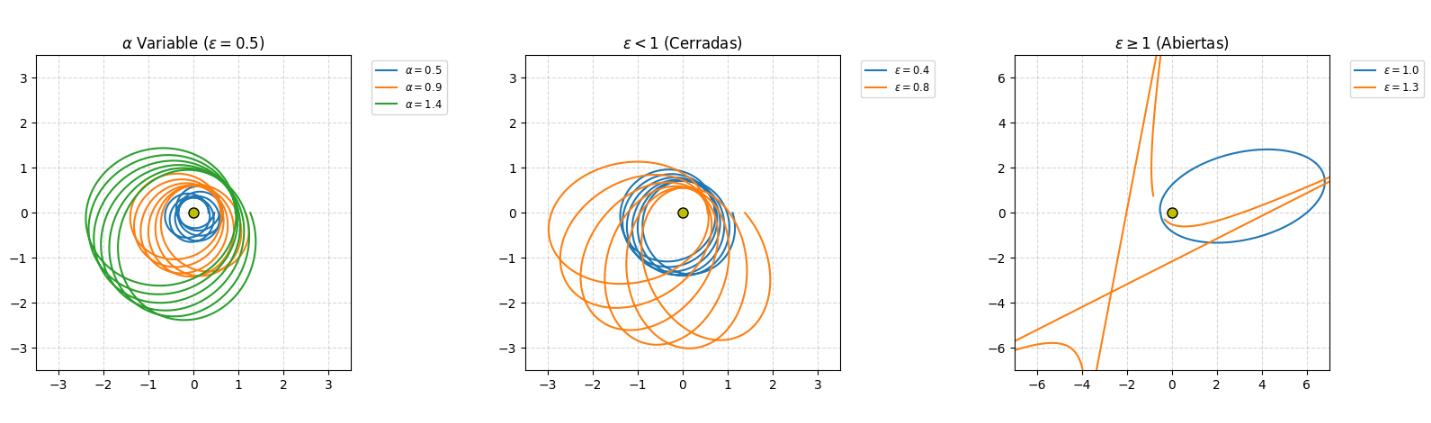
\includegraphics[width=1\textwidth]{figuras/variacion_re_coord_cartesianas.png}
		\caption{Variación de parámetros en el modelo relativista.}
	\end{figure}
	\newpage
	
	\textbf{Comparativa entre el modelo clásico de Kepler y la corrección relativista}
	\\
	
	Al incorporar el término no lineal de perturbación $\delta > 0$ al sistema (que introduce una dependencia con la inversa del cubo de la distancia), observamos de manera inmediata que las trayectorias ya no definen una elipse perfecta. Es decir, pierden la periodicidad estricta de $2\pi$ en el ángulo orbital. 
	
	Para un valor de $\delta = 0.05$, la trayectoria pasa a describir lo que visualmente se asemeja a una flor, formalmente conocida como órbita de roseta. En términos del perihelio, vemos un desplazamiento progresivo del punto de mínima distancia radial; la trayectoria necesita un ángulo mayor a $2\pi$ para volver a este punto crítico, perdiendo así su capacidad de definir una órbita espacialmente cerrada en un solo ciclo. Este fenómeno astronómico es el que se conoce como la "precesión del perihelio", el cual fue correctamente descrito para la órbita de Mercurio gracias a la corrección relativista.
	
	Al observar el espacio de fases ($u$ frente a $\dot{u}$), el sistema sigue manteniendo un comportamiento periódico en sus variables de estado, el planeta sigue oscilando de forma estable entre un máximo y un mínimo de distancia, por lo que seguimos viendo una elipse. Sin embargo, en el caso relativista, esta elipse se percibe un poco más pequeña respecto a la clásica. Esto ocurre porque el término de perturbación $\delta u^2$ introduce una atracción adicional en el sistema. Otra consecuencia visible es que en el modelo de Kepler, para $\epsilon = 1$ obtenemos una trayectoria parabólica de escape, sin embargo, aquí el sistema no cuenta con la energía suficiente para vencer la atracción extra, resultando en una órbita ligada.
	
	\begin{figure}[htbp]
		\centering
		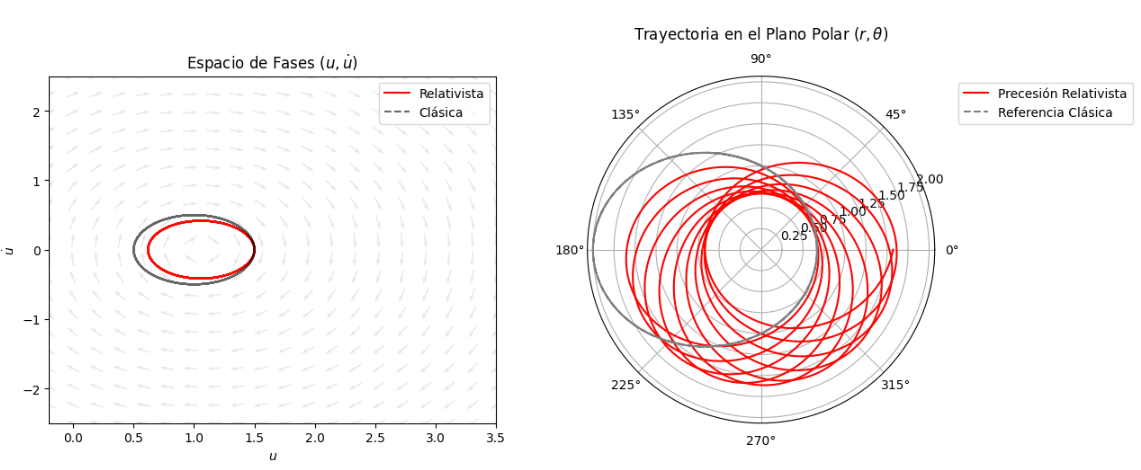
\includegraphics[width=0.9\textwidth]{figuras/comparacion_re_coord_polares.png}
		\caption{Comparación entre el modelo clásico (Kepler) y el modelo relativista.}
	\end{figure}
	
\end{document}